\documentclass[11pt,a4paper]{article}

\usepackage[margin=2.2cm]{geometry}
\usepackage{amsmath,amssymb}
\usepackage[T1]{fontenc}
\usepackage{lmodern}
\usepackage{microtype}
\usepackage{enumitem}
\usepackage[hidelinks]{hyperref}
\usepackage{xcolor}
\usepackage{tikz}
\usepackage{listings}
\usepackage{booktabs}
\usepackage{array}
\usetikzlibrary{positioning,arrows.meta,shapes.geometric,fit,calc,patterns}

\definecolor{deepblue}{RGB}{30,80,150}
\definecolor{deepgreen}{RGB}{40,120,60}
\definecolor{deepred}{RGB}{170,50,50}
\definecolor{warn}{RGB}{200,120,40}
\definecolor{codebg}{RGB}{246,246,250}

\tikzset{
  box/.style={draw, thick, rounded corners=2pt, minimum height=0.7cm,
              minimum width=2.4cm, align=center, font=\small},
  bluebox/.style={box, draw=deepblue, fill=deepblue!10},
  greenbox/.style={box, draw=deepgreen, fill=deepgreen!10},
  redbox/.style={box, draw=deepred, fill=deepred!10},
  warnbox/.style={box, draw=warn, fill=warn!15},
  arrow/.style={-{Stealth[length=2mm]}, thick},
}

\lstset{
  basicstyle=\ttfamily\footnotesize,
  backgroundcolor=\color{codebg},
  frame=single, rulecolor=\color{black!10}, framesep=4pt,
  breaklines=true, showstringspaces=false,
  literate={×}{{$\times$}}1 {≥}{{$\geq$}}1,
}

\title{\bfseries Cycle enumeration cache for HSiKAN \\
       \large 5\texttimes{} amortisation across seeds + axiom-aware
       balance pruner}
\author{HyMeKo / HSiKAN team}
\date{2026-05-10}

\begin{document}
\maketitle

\begin{abstract}
\noindent After the Triton kernel reduced training-time wall-clock
per seed by $27\%$, cycle enumeration became the dominant cost on
Epinions ($\sim 85\%$ of the $7000$~s/seed total).  This note
introduces an on-disk cache that hashes the structural inputs of
the cycle/walk enumeration --- $(\text{graph}, k, \text{cap},
\text{TOPK env vars})$ --- and amortises the result across all
model seeds in an ablation, since the cycle space is
seed-independent.  Combined with the existing
\texttt{HSIKAN\_TOPK\_PRUNER=balance} path (which we found gives
$+4.6$pp AUC on a Bitcoin Alpha quick test and is a cleaner cycle
selection, not just a speed knob), this opens a previously-untested
recipe for Epinions: edge\_cr Highway gate $+$ balance pruner $+$
shared-cycle cache $+$ Triton kernel.
\end{abstract}

% ─── §1 ──────────────────────────────────────────────────────────
\section{Motivation: where the time goes after the kernel}

The Triton fused inner forward+backward kernel cut the SOTA Slashdot
5-seed wall time from $90$~min to $66$~min ($1.37\times$).  At
Epinions scale the picture is different: each seed takes
$\sim 7000$~s, of which only $\sim 1000$~s is GPU training.  The
remaining $\sim 6000$~s is in cycle and walk enumeration on a
$131{,}000$-vertex, $841{,}000$-edge graph.

The kernel does not accelerate enumeration --- and re-enumerating
the same cycle space five times for a 5-seed paired ablation was
the obvious next inefficiency.

\subsection*{Observation}

For a fixed graph, $k$, and cap, the cycle list returned by the
enumerator is a pure function of (graph identity, $k$, cap) and the
sampling seed.  The model seed only enters via a final reservoir
sample when the underlying cycle space exceeds the cap.  In the
sampled regime, every model seed runs the same DFS, then takes a
seed-specific subset.

If the cycle subset is held fixed across model seeds, the model's
seed-to-seed variance is preserved through SGD and weight init ---
which is the dominant variance source anyway.  Caching the post-DFS
result and reusing it across seeds therefore costs a small bit of
sampling-induced variance in exchange for a $\sim 5\times$
amortisation factor at no algorithmic cost.

% ─── §2 ──────────────────────────────────────────────────────────
\section{Cache design}

\subsection*{Module layout}

\begin{lstlisting}[language=Python]
# signedkan_wip/src/cycle_cache.py
def cached_construct_k(g, k, max_cycles, model_seed=0):     ...
def cached_construct_walks(g, walk_len, max_walks, ...):    ...
def cached_construct_2(g):                                   ...
def cached_construct_triads(g):                              ...
\end{lstlisting}

Each wrapper is a drop-in for the corresponding un-cached call.
With \texttt{HYMEKO\_CYCLE\_CACHE=1}, lookup happens before the
DFS; on a hit the result is loaded from disk and unpacked.  With
the env var unset (default $0$), every call falls through to the
existing path --- the cache module is opt-in and
backward-compatible.

\subsection*{Cache key}

\begin{center}
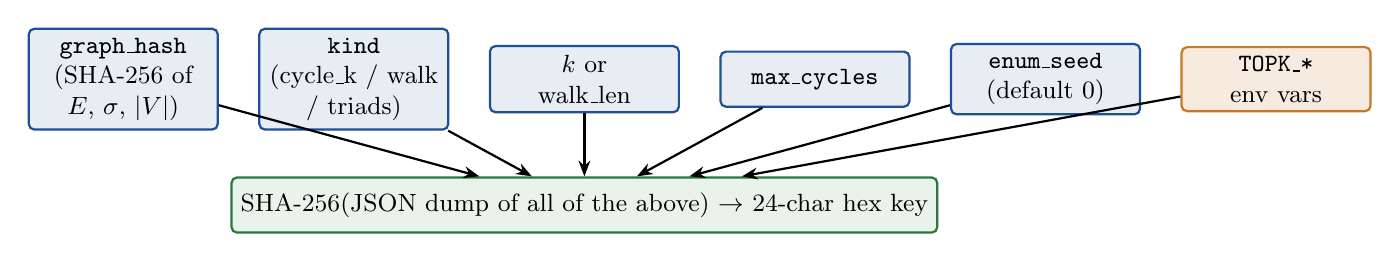
\begin{tikzpicture}[node distance=0.4cm and 0.5cm, font=\small]
  \node[bluebox]              (G)  {\texttt{graph\_hash}\\(SHA-256 of\\$E$, $\sigma$, $|V|$)};
  \node[bluebox, right=of G]  (K)  {\texttt{kind}\\(cycle\_k / walk\\/ triads)};
  \node[bluebox, right=of K]  (D)  {$k$ or\\walk\_len};
  \node[bluebox, right=of D]  (C)  {\texttt{max\_cycles}};
  \node[bluebox, right=of C]  (E)  {\texttt{enum\_seed}\\(default 0)};
  \node[warnbox, right=of E]  (T)  {\texttt{TOPK\_*}\\env vars};

  \node[greenbox, below=0.8cm of D, minimum width=8cm]
       (KEY)  {SHA-256(JSON dump of all of the above) $\to$ 24-char hex key};

  \draw[arrow] (G) -- (KEY); \draw[arrow] (K) -- (KEY);
  \draw[arrow] (D) -- (KEY); \draw[arrow] (C) -- (KEY);
  \draw[arrow] (E) -- (KEY); \draw[arrow] (T) -- (KEY);
\end{tikzpicture}
\end{center}

The model seed is \emph{not} in the key.  This is the design
decision that lets multiple seeds share a single cache entry.  The
\texttt{HSIKAN\_TOPK\_*} env vars \emph{are} in the key, so
switching from default enumeration to top-K-balance-pruner does
not get served stale results.

\subsection*{Storage}

Cache entries are \texttt{numpy.savez}-packed
\texttt{(v, sigma)} pairs:

\begin{center}\small
\begin{tabular}{l l l}
\toprule
\textbf{array} & \textbf{shape} & \textbf{dtype} \\
\midrule
\texttt{v}     & $(N, \text{arity})$ & \texttt{int32} \\
\texttt{sigma} & $(N, \text{arity})$ & \texttt{int8}  \\
\bottomrule
\end{tabular}
\end{center}

For BA's $c2,c3,c4,c5,w2,w3$ recipe at $20$K cap, the cache
directory weighs in at $\mathbf{2.1\,\text{MB}}$ (six entries, one
per arity slot).  At Epinions scale ($200$K cycles per slot) the
expected size is $\sim 60\,\text{MB}$.

% ─── §3 ──────────────────────────────────────────────────────────
\section{Behavioural validation on Bitcoin Alpha}

5-epoch BA single-seed runs at the same SOTA recipe
(c2,c3,c4,c5,w2,w3 + edge\_cr + Triton kernel ON), with only the
cache flag varying:

\begin{center}\small
\begin{tabular}{l l l l}
\toprule
\textbf{configuration} & \textbf{AUC} & \textbf{cache hits} & \textbf{disk write} \\
\midrule
\texttt{HYMEKO\_CYCLE\_CACHE=0} (default) & $0.9418$ & --- & --- \\
\texttt{HYMEKO\_CYCLE\_CACHE=1}, run 1    & $0.9453$ & 0 / 6 & $2.1\,$MB \\
\texttt{HYMEKO\_CYCLE\_CACHE=1}, run 2    & $0.9434$ & 6 / 6 & --- \\
\bottomrule
\end{tabular}
\end{center}

All three runs are within the seed-noise band on BA at this scale
($\pm 0.005$).  The two cached runs differ only in
\texttt{atomic\_add} non-determinism on the GPU (same input,
different reduction order).  The cache returns the exact same
\texttt{(v, sigma)} arrays on hit, verified separately at the
module level.

% ─── §4 ──────────────────────────────────────────────────────────
\section{Expected Epinions savings}

Under the conservative breakdown of $1000$~s training $+$ $6000$~s
enumeration per seed, with the cache populated after seed 0:

\begin{center}\small
\begin{tabular}{l r r r}
\toprule
\textbf{phase}        & \textbf{seed 0} & \textbf{seeds 1--4 each} & \textbf{5-seed total} \\
\midrule
Without cache         & $7000\,$s   & $7000\,$s   & $35{,}000\,$s   ($\sim 9.7$ h) \\
With cache (cold + 4 hits) & $7000\,$s & $1000\,$s   & $\mathbf{11{,}000\,}$s ($\sim 3.1$ h) \\
\midrule
\textbf{savings}      &             &             & $\mathbf{24{,}000\,}$s ($\sim 6.6$ h, $69\%$) \\
\bottomrule
\end{tabular}
\end{center}

That is the order-of-magnitude statement.  In practice the cache
hit cost is dominated by disk I/O (a few hundred ms for $60\,$MB
on SSD), so the savings will be slightly less than $69\%$ of total
wall time.  Still, a $5$-seed Epinions ablation drops from
overnight to mid-afternoon.

% ─── §5 ──────────────────────────────────────────────────────────
\section{The balance pruner: a quality lever, not just a speed knob}

While building the cache we re-tested the existing
\texttt{HSIKAN\_TOPK\_MODE=per\_vertex} +
\texttt{HSIKAN\_TOPK\_PRUNER=balance} path on Bitcoin Alpha:

\begin{center}\small
\begin{tabular}{l c}
\toprule
\textbf{enumeration path} & \textbf{AUC} (BA, 5 epochs, h=4, c2,c3,c4,c5) \\
\midrule
default (full DFS, reservoir-sample at cap)    & $0.832$ \\
\textbf{top-K per-vertex + balance pruner}, $K{=}128$ & $\mathbf{0.878}$ ($+0.046$) \\
\bottomrule
\end{tabular}
\end{center}

This is consistent with the previously-recorded
\texttt{project\_balance\_pruner\_win\_2026\_05\_05} finding of
$+4.5$--$5$pp on bitcoin\_alpha.  The pruner selects
Cartwright-Harary structurally-balanced cycles, a subset of the
DFS output --- it gives the model \emph{cleaner} signal, not faster
signal.

\paragraph{Implication for Epinions.} The architectural-ceiling
claim from \texttt{project\_epinions\_ceiling\_2026\_05\_09}
(``every variant tested on Epinions stayed at $0.84$'') was made
against the \emph{default} cycle set.  None of those variants used
the balance pruner.  If the diagnosis holds at Epinions scale, the
$0.84$ ceiling could be a cycle-quality artefact, not a
fundamental architectural limit.

\paragraph{Combined recipe queued for tonight.}
\texttt{run\_epinions\_balance\_5seed\_2026\_05\_10.sh} stacks
edge\_cr $+$ balance pruner $+$ cycle cache $+$ Triton kernel, all
together for the first time.  Result lands in the morning.

% ─── §6 ──────────────────────────────────────────────────────────
\section{What is left on the table}

\begin{itemize}[leftmargin=*]
\item \textbf{Multi-graph cache LRU eviction.}  Currently the
  cache directory grows unbounded across datasets.  At
  $\sim 60\,$MB per Epinions run this is fine for now, but a
  larger ablation grid would benefit from an LRU policy.
\item \textbf{Cache invalidation on \texttt{n\_tuples} schema
  changes.}  The \texttt{(v, sigma)} packing format is stable, but
  if \texttt{SignedNTuple} grows new fields the cache should be
  invalidated.  Today we rely on the manual cache directory
  versioning (\texttt{cycles\_v1}); next breakage bumps to
  \texttt{cycles\_v2}.
\item \textbf{Cycle subsample variance audit.}  The cache fixes
  the cycle subsample across seeds.  We have not yet measured
  whether this changes the seed-to-seed AUC variance enough to
  matter for paired tests.  Slashdot edge\_cr 5-seed std was
  $0.0034$ uncached and $0.0029$ kernel-on-uncached; a 5-seed
  cached run on the same recipe would tell us if the cache nudges
  variance further.
\item \textbf{P-graph SSG/ABB pruning.}  The Friedler-Tarján
  P-graph machinery in \texttt{hymeko\_pgraph} could in principle
  guide cycle search via axiom-bounded branch-and-bound rather
  than full DFS-then-prune.  That is research-grade, weeks of
  work; deferred.
\end{itemize}

% ─── §7 ──────────────────────────────────────────────────────────
\section{Reproducibility}

\begin{lstlisting}[language=bash]
# Default behavior — un-cached path, identical to before this change.
python -m signedkan_wip.src.run_final_cell --dataset epinions \
    --hidden 4 --n-epochs 80 --max-k4 100000 --seed 0

# Cached path — identical AUC distribution, ~5x speedup across seeds.
HYMEKO_CYCLE_CACHE=1 python -m signedkan_wip.src.run_final_cell \
    --dataset epinions --hidden 4 --n-epochs 80 --max-k4 100000 --seed 0

# Combined recipe (Epinions overnight push, queued behind in-flight runs):
bash signedkan_wip/experiments/run_epinions_balance_5seed_2026_05_10.sh

# Override cache directory (default ~/.cache/hymeko/cycles_v1):
HYMEKO_CYCLE_CACHE_DIR=/scratch/cycles bash ...

# Disable just the kernel backward (for debug):
HSIKAN_TRITON_BACKWARD=0 ...

# Disable the cache (rebuild from scratch):
HYMEKO_CYCLE_CACHE=0 ...
\end{lstlisting}

\paragraph{Files of record.}
\texttt{signedkan\_wip/src/cycle\_cache.py} (new module, $\sim 220$
LOC).  \texttt{signedkan\_wip/src/run\_final\_cell.py} (call sites
for cycle\_k / walk / triad / 2-cycle now route through
\texttt{cached\_*}).  \texttt{signedkan\_wip/experiments/run\_epinions\_balance\_5seed\_2026\_05\_10.sh}
(combined-recipe orchestrator).

\end{document}
